\section{Library Evaluation}

This section presents preliminary evaluation results of the TAkka library.  
We show that the Wadler's type pollution problem can be strateforwardly avoided by in TAkka.   
We further assess the TAkka library by porting examples built in Erlang and Akka.  The
result shows that TAkka is able to detect more forms of type errors without
obvious overheads.


\subsection{Wadler\rq{}s Type Pollution Problem}
\label{type_pollution}

Wadler\rq{}s type pollution problem refers to the situation where the same
communication interface is published to two or more parties for distinct
purposes.  In a system suffers from the type pollution problem, a service
provider may receive a request that is not expected from the requester.
Examples of type polluted systems are those constructed using the layered
architecture or the MVC model without due care.

One solution to the type pollution problem is using separate channels for
distinct parties.  Programming models that supports this solution includes
join-calculus \cite{full_join} and session types\cite{Honda_languageprimitives}.

The other solution to the type pollution problem is using sub-typing.  Take a
layered architecture system for example. Let {\bf UpperMsg} and {\bf LowerMsg}
be the type of messages expected from the upper layer and the lower layer
respectively.  Both {\bf UpperMsg} and {\bf LowerMsg} are subtypes of {\bf
MiddleMsg}, the least general type of messages expected by the middle layer.
In the code below, the middle layer publishes itself as different types to the
upper layer and the lower layer.  Therefore, neither the upper layer nor the
lower layer is aware of the communication interface between the other
layer and the middle layer.

\begin{lstlisting}
sealed trait MiddleMsg
class UpperMsg extends MiddleMsg
class LowerMsg extends MiddleMsg

class UpperLayer {
  private var middle:ActorRef[UpperMsg]
  def setMiddleLayer(mid:ActorRef[UpperMsg]) = {
    this.middle = mid
}}
class LowerLayer {
  private var middle:ActorRef[LowerMsg]
  def setMiddleLayer(mid:ActorRef[LowerMsg]) = {
    this.middle = mid
}}

class MiddleLayer extends Actor[MiddleMsg] {
  val upper:UpperLayer
  val lower:LowerLayer

  upper.setMiddleLayer(typedSelf)
  lower.setMiddleLayer(typedSelf)
  // rest of initialization code
}
\end{lstlisting}

\subsection{Expressiveness and Correctness}

Table-\ref{express} lists examples used for expressiveness and correctness test.
We selected examples from Akka and other OTP projects and re-implement them  in
TAkka to ensure that main requirements for actor programming are not
unintentionally neglected.  The reported results show that when porting an Akka
program to TAkka, new type declarations will be added to about 12\% lines of
code; Meanwhile, because TAkka actors do not need to handle unexpected messages,
the total program size of Akka and TAkka applications are almost the same.

A type error is reported by the compiler when porting the Socko example
\cite{SOCKO} from its Akka implementation to equivalent TAkka implementation.
SOCKO is a library for building event-driven web services.  The SOCKO designer
defines a {\bf SockoEvent} class to be the supertype of all events.  One
subtype of {\bf SockoEvent} is {\bf HttpRequestEvent}, representing events
generated when an HTTP request is received. The designer further implements
subclasses of {\bf Method}, whose {\it unapply} method intends to pattern
matching {\bf SockoEvent} to {\bf HttpRequestEvent}.  Somehow, the SOCKO
designer made a type error in the method declaration so that the {\it unapply}
method pattern matches {\bf SockoEvent} to {\bf SockoEvent}. The type error is
not exposed in test examples because the designer always passes instances of
{\bf HttpRequestEvent} to the {\it unapply} method and send the the returned
values to an actor that accepts messages of {\bf HttpRequestEvent} type.
Fortunately, such ill-typed message is not accepted in TAkka, even if the code
may or may not work.

\begin{table}[h]
\label{express}
% \tbl{Examples for Correctness and Expressiveness Test}{
\caption{Examples for Correctness and Expressiveness Test}
  \begin{adjustwidth}{-1.8cm}{}
\begin{tabular}{| l | c | c | c |  c | c | c |}
\hline

Source & Example & \specialcell{Akka\\ Code Lines} &
\specialcell{Modified\\ TAkka Lines} & \specialcell{\% of \\Modified Code} &
\specialcell{TAkka\\Code Lines}
& \specialcell{\% of \\Code Size} \\
\hline
Quviq\cite{quviq}  & ATM simulator & 1148 & 199 & 17.3 & 1160 & 101 \\
\cline{2-7}
                   & Elevator Controller &
2850 & 172 & 9.3 & 2878 & 101 \\
\hline


                   & Ping Pong & 67 & 13 & 19.4 & 67 & 100 \\
\cline{2-7}
Akka   & Dining Philosophers &
189 & 23 & 12.1 &
189 & 100  \\
\cline{2-7}
Documentation\cite{akka_doc}  & Distributed Calculator  & 250 &
43 & 17.2 & 250 & 100 \\
\cline{2-7}
                                   & Fault Tolerance & 274 & 69 & 25.2 & 274 &
100 \\
\hline

                                   & Barber Shop\cite{BarberShop} & 754 & 104 &
13.7 & 751 & 99 \\
\cline{2-7}
Other Open & EnMAS \cite{EnMAS} & 1916 & 213
& 11.1 & 1909 &
100 \\
\cline{2-7}
Source Akka        & Socko Web Server \cite{SOCKO} & 5024 & 227
& 4.5 & 5017 & 100 \\
\cline{2-7}
Applications                                          & Gatling \cite{Gatling} 
& 1635 & 111 & 6.8 & 1623 & 99\\
\hline
geometric mean                   & & 712.4 & 83.7 & 12.2 & 712.7 & 100.0 \\
\hline
\end{tabular}
% }
  \end{adjustwidth}
\end{table}




\subsection{Efficiency and Scalability Evaluation}
The TAkka library is build on top of Akka so that code for shared features could
be re-used.  The three main overheads of the TAkka implementation are: (i) the
cost of adding an additional operation layer on top of Akka code, (ii) the cost
of constructing {\bf Manifest}, and (iii) the cost of transmitting {\bf
Manifest} in distributed settings.  The cost of the last factor is subject to
network connections.  We access the upper bound of the cost of the first two
factors by accessing the time of initializing {\it n} instances of {\bf MyActor}
defined in \S\ref{akka actor} and \S\ref{actor_ref}.  When {\it n} ranges from
$10^4$ to $10^5$, the time measurement TAkka implementation is about 30\% more
than the time measurement of Akka implementation.

We further investigated the efficiency and scalability of TAkka by porting
9 examples from the BenchErl benchmarks in the RELEASE project \cite{RELEASE}.
The benchmarks are run on a Beowulf cluster at the Heriot-Watt University.
The 32 Beowulf cluster nodes each comprise eight Intel 5506 cores running at
2.13GHz. All machines running under Linux CentOS 5.5. The Beowulf nodes are
connected with Baystack 5510-48T switch with 48 10/100/1000 ports.  

Figure \ref{scalability} gives the result of three representative benchmarks: MBrot,
RUN, and SerialMsg. Each benchmark spawns one master process and many child
processes.  The child process performs a certain amount of calculation and
reports the result to the master process.  The MBrot example requires heavy
calculation in each child process.  The RUN example requires a small amount of
calculation in each child process.  The SerialMsg example ask each child forward
messages. The result shows that TAkka and Akka have almost identical run-time performance and scalability.  For all 3 examples in Figure \ref{scalability}, TAkka is never more than 10.5\% slower than Akka.

\begin{figure}[h]
     \begin{center}
        \subfigure[]{
            \label{fig:first}
            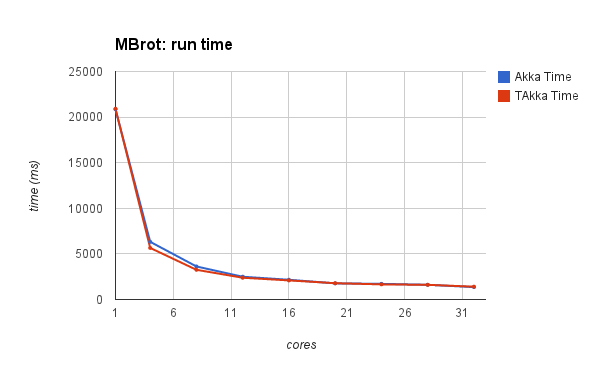
\includegraphics[scale=0.33]{MBrot_time.png}
        }
        \subfigure[]{
           \label{fig:second}
           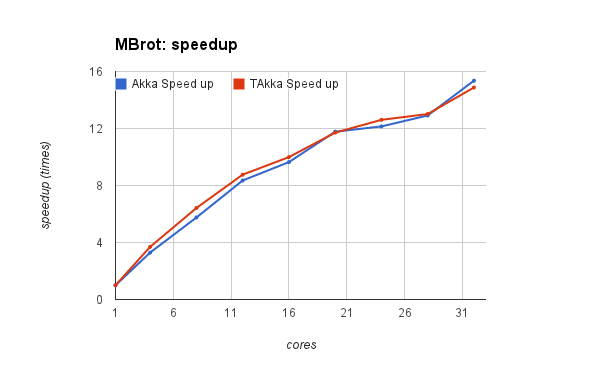
\includegraphics[scale=0.33]{MBrot_speedup.png}
        }\\
        \subfigure[]{
            \label{fig:third}
            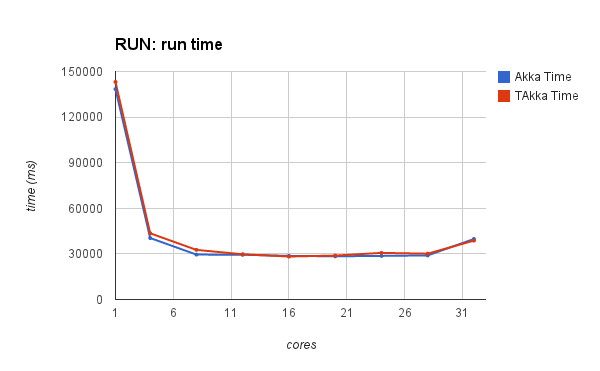
\includegraphics[scale=0.33]{RUN_time.png}
        }
        \subfigure[]{
            \label{fig:fourth}
            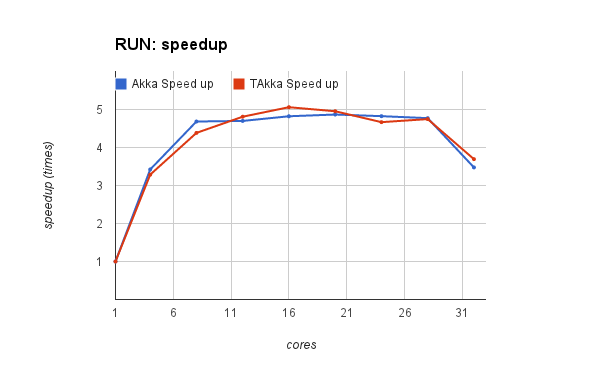
\includegraphics[scale=0.33]{RUN_speedup.png}
        }\\
        \subfigure[]{%
            \label{fig:fifth}
            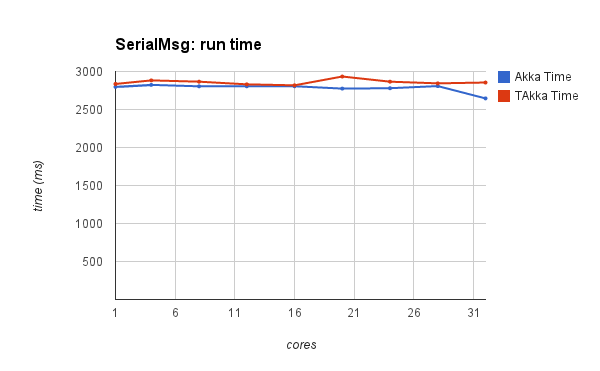
\includegraphics[scale=0.33]{SerialMsg_time.png}
        }
        \subfigure[]{%
            \label{fig:sixth}
            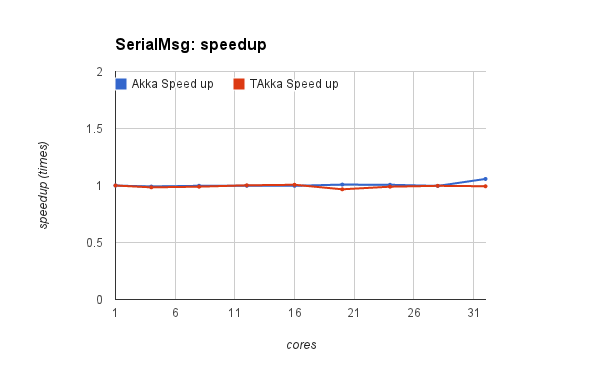
\includegraphics[scale=0.33]{SerialMsg_speedup.png}
        }\\
    \end{center}
    \caption{Efficiency and Scalability Benchmark}
   \label{scalability}
\end{figure}
